% Character-level name generation — assignment report
% Compile: pdflatex report.tex   (run twice if you add \ref/\cite later)
\documentclass[11pt,a4paper]{article}

\usepackage[utf8]{inputenc}
\usepackage[T1]{fontenc}
\usepackage{lmodern}
\usepackage[a4paper,margin=2.5cm]{geometry}
\usepackage{amsmath,amssymb}
\usepackage{booktabs}
\usepackage{graphicx}
\usepackage{hyperref}
\usepackage{listings}
\usepackage{xcolor}
\usepackage{caption}
\usepackage{enumitem}

\hypersetup{
  colorlinks=true,
  linkcolor=blue!60!black,
  urlcolor=blue!60!black,
  citecolor=blue!60!black,
}

\lstset{
  basicstyle=\ttfamily\small,
  breaklines=true,
  frame=single,
  backgroundcolor=\color{gray!8},
  keywordstyle=\color{blue!70!black},
}

\title{\textbf{Problem 2: Character-Level Indian Name Generation\\
Using RNN Variants}\\[0.4em]
\large Vanilla RNN, Bidirectional LSTM, RNN with Attention (PyTorch)}
\author{%
  \textbf{Shivam Madhav Kenche}\\
  Roll No.: \texttt{M25CSA028}%
}
\date{\today}

\begin{document}
\maketitle

\begin{abstract}
This report describes dataset construction, three recurrent architectures for
next-character prediction, quantitative metrics (novelty rate and diversity), and
qualitative analysis of generated Indian-style names. Implementations use PyTorch;
BLSTM uses prefix-aligned training and prefix decoding; the attention model uses
causal prefix pooling and prefix decoding for aligned inference.
\end{abstract}

\tableofcontents
\bigskip

% ---------------------------------------------------------------------------
\section{Task 0: Dataset}
% ---------------------------------------------------------------------------
Names were collected into \texttt{TrainingNames.txt} (one name per line), targeting
at least 1000 Indian given names via an LLM-assisted script (\texttt{generate\_dataset.py})
with multiple regional/demographic prompts, deduplication, and light cleaning.

\begin{table}[h]
  \centering
  \caption{Dataset summary (see repository for full details).}
  \begin{tabular}{ll}
    \toprule
    Property & Value \\
    \midrule
    Total names & 1\,076 \\
    File & \texttt{TrainingNames.txt} \\
    Approx.\ mean length & $\sim$7 characters \\
    \bottomrule
  \end{tabular}
\end{table}

% ---------------------------------------------------------------------------
\section{Task 1: Models and training}
% ---------------------------------------------------------------------------
All models perform character-level language modelling with teacher forcing:
input sequence $\langle\texttt{SOS}\rangle, c_1,\ldots,c_n$ and targets
$c_1,\ldots,c_n,\langle\texttt{EOS}\rangle$. Vocabulary includes
\texttt{PAD}, \texttt{SOS}, \texttt{EOS} and all characters in the training set
(vocabulary size $\approx 55$ in this run).

\subsection{Vanilla RNN}
Embedding ($d=64$) $\rightarrow$ \texttt{nn.RNN} ($h=256$, 2 layers, dropout 0.3)
$\rightarrow$ linear to vocabulary. \textbf{Trainable parameters:} 231\,671.

\subsection{Bidirectional LSTM (BLSTM)}
Embedding ($d=64$) $\rightarrow$ \texttt{nn.LSTM} bidirectional ($h=128$ per direction,
2 layers, dropout 0.3) $\rightarrow$ linear ($2h \rightarrow |V|$).
Training uses \emph{causal prefix loss} (see \texttt{train.py}): at each position the
loss is computed from a forward pass on the prefix only, matching decoding.
Generation uses \emph{prefix re-encoding} each step.
\textbf{Trainable parameters:} 611\,575.

\subsection{RNN with additive attention}
Embedding $\rightarrow$ \texttt{nn.RNN} ($h=256$, 2 layers) $\rightarrow$ at each time
step $t$, additive (Bahdanau-style) attention over hidden states $h_0,\ldots,h_t$ only
(causal), concatenated with $h_t$, then linear to vocabulary. Decoding uses the same
prefix re-encoding as BLSTM.
\textbf{Trainable parameters:} 311\,799.

\subsection{Shared hyperparameters}
Adam optimizer, learning rate $10^{-3}$, batch size 32, gradient clip norm 1.0,
\texttt{ReduceLROnPlateau} scheduler, early stopping (patience 15), up to 100 epochs.
Training/validation split: 90\%/10\%.

% Optional: uncomment if PDF and images live next to this .tex file
% \begin{figure}[h]
%   \centering
%   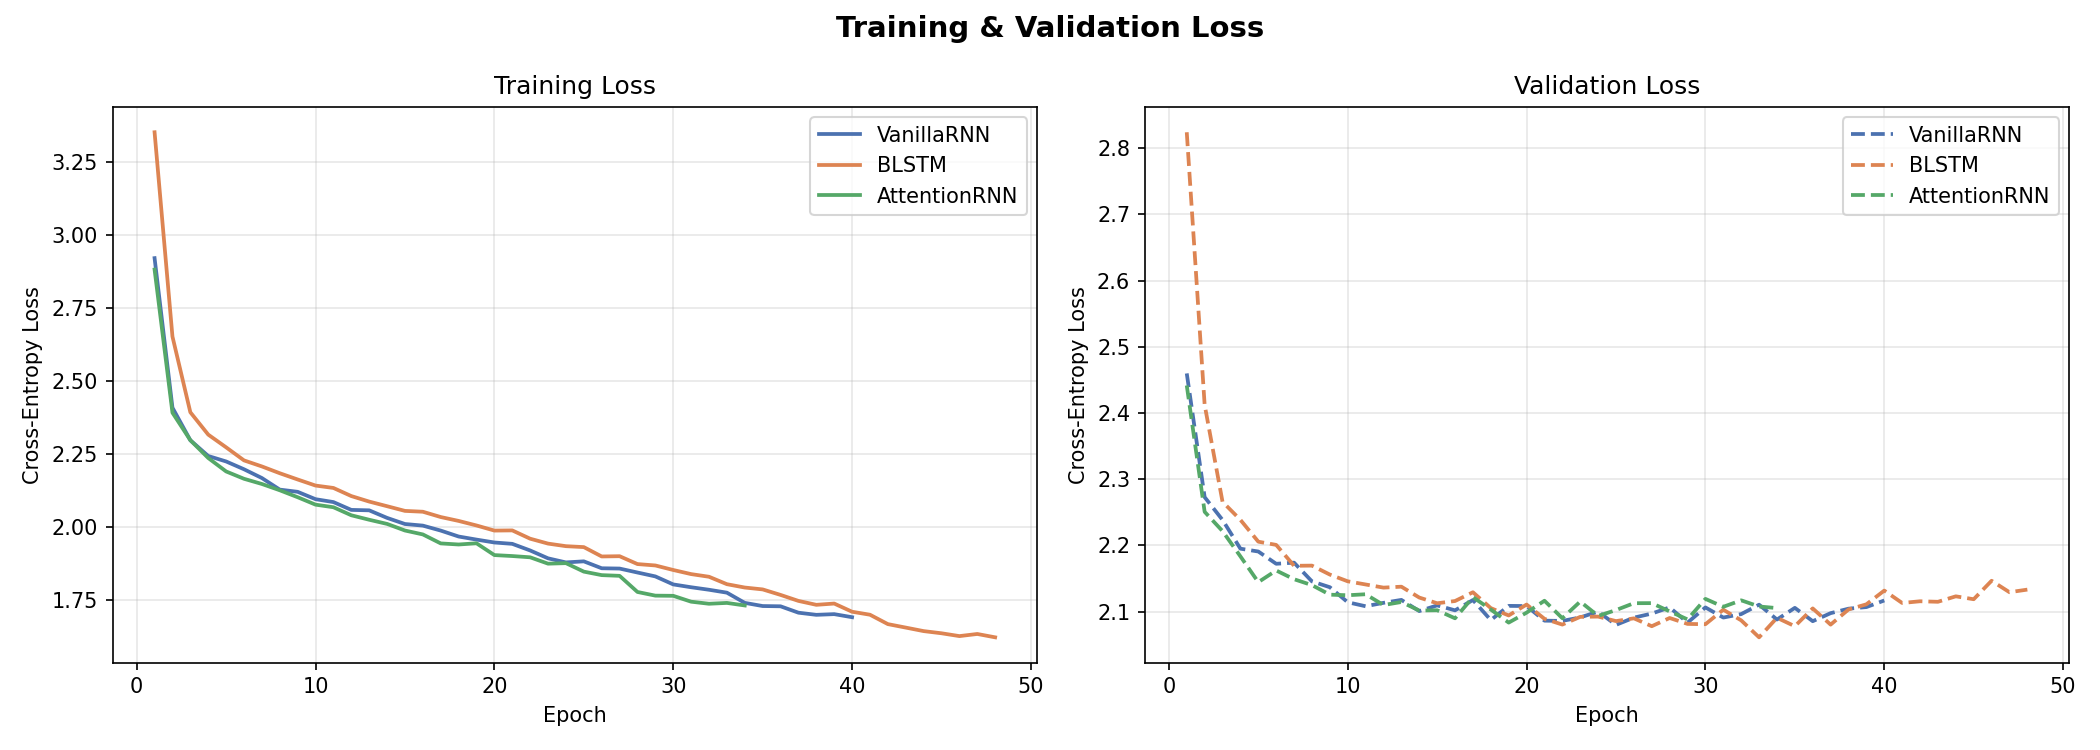
\includegraphics[width=0.95\linewidth]{results/loss_curves.png}
%   \caption{Training and validation loss (from \texttt{plot\_results.py}).}
% \end{figure}

% ---------------------------------------------------------------------------
\section{Task 2: Quantitative evaluation}
% ---------------------------------------------------------------------------
For each model, 200 names were generated with temperature $0.8$.
Metrics (from \texttt{evaluate.py}, stored in \texttt{results/evaluation\_results.json}):

\begin{itemize}[nosep]
  \item \textbf{Novelty rate:} percentage of generated names not present in the training set (case-insensitive).
  \item \textbf{Diversity:} (number of unique generated strings) / (total generated).
\end{itemize}

\begin{table}[h]
  \centering
  \caption{Measured metrics on the evaluation run archived in the repository JSON.}
  \label{tab:metrics}
  \begin{tabular}{lcccc}
    \toprule
    Model & Novelty (\%) & Diversity & Avg.\ len.\ ($\pm$ std) & Char.\ coverage \\
    \midrule
    VanillaRNN   & 92.0 & 0.975 & $6.37 \pm 1.39$ & 0.9615 \\
    BLSTM        & 90.5 & 0.985 & $6.43 \pm 1.57$ & 1.0000 \\
    AttentionRNN & 92.0 & 0.990 & $6.86 \pm 1.82$ & 1.0000 \\
    \bottomrule
  \end{tabular}
\end{table}

\noindent
\textbf{Note:} Re-running \texttt{generate\_names.py} resamples from the models, so
novelty and diversity can shift slightly; re-run \texttt{evaluate.py} for a consistent
table before final submission.

% Uncomment when metrics figure exists beside this file:
% \begin{figure}[h]
%   \centering
%   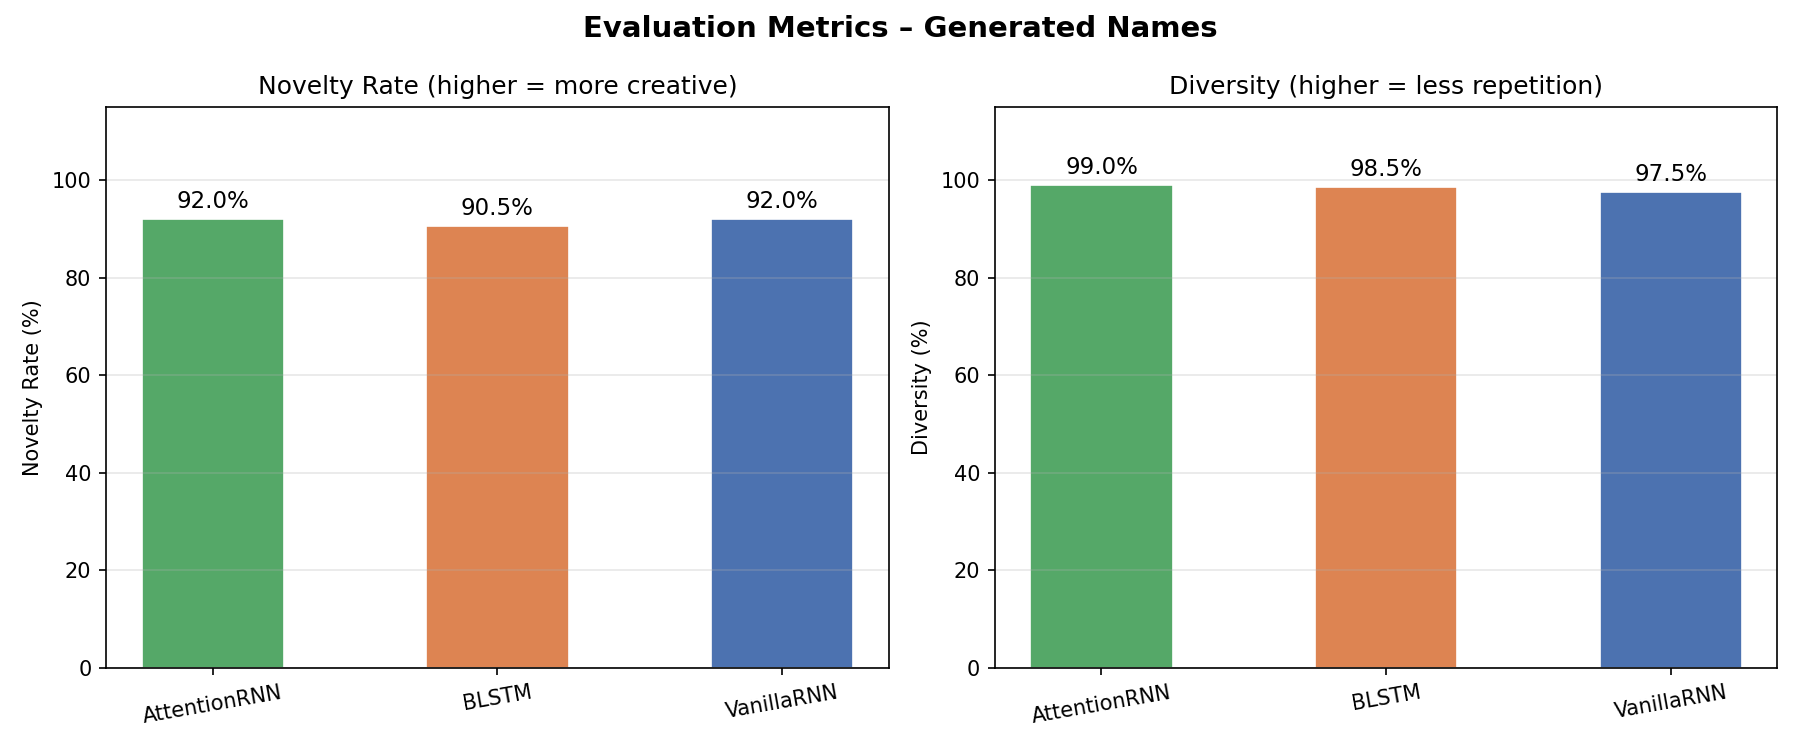
\includegraphics[width=0.95\linewidth]{results/metrics_comparison.png}
%   \caption{Bar plot of novelty and diversity (\texttt{plot\_results.py}).}
% \end{figure}

% ---------------------------------------------------------------------------
\section{Task 3: Qualitative analysis}
% ---------------------------------------------------------------------------
\subsection{Realism}
All three models produce short strings that read like plausible Indian given names
(blends of common stems and endings), with occasional misspellings or unlikely
consonant clusters typical of small character-level LMs.

\subsection{Representative samples}
Examples from \texttt{generated/} (same evaluation run as Table~\ref{tab:metrics}):

\paragraph{VanillaRNN.}
\texttt{Suthan}, \texttt{Amutra}, \texttt{Umayal}, \texttt{Anindi}, \texttt{Amisha},
\texttt{Teeta}, \texttt{Amarti}, \texttt{Amaraman}, \texttt{Ramindean}, \texttt{Aljitsan}.

\paragraph{BLSTM.}
\texttt{Shureth}, \texttt{Naedeep}, \texttt{Darpan}, \texttt{Sharamti}, \texttt{Sooni},
\texttt{Sumar}, \texttt{Aanya}, \texttt{Prija}, \texttt{Bhavekh}, \texttt{Jetya}.

\paragraph{AttentionRNN.}
\texttt{Ramanira}, \texttt{Onkav}, \texttt{Darvipree}, \texttt{Rajan}, \texttt{Veera},
\texttt{Anna}, \texttt{Hertendra}, \texttt{Amandik}, \texttt{Sunal}, \texttt{Mohif}.

\subsection{Failure modes}
\begin{itemize}[nosep]
  \item Rare early \texttt{EOS}: very short outputs.
  \item Odd spellings or consonant clusters: limited data and sampling noise.
  \item High temperature increases randomness and garbage substrings.
\end{itemize}

% ---------------------------------------------------------------------------
\section{Conclusion}
% ---------------------------------------------------------------------------
Vanilla RNN, causal BLSTM with prefix training/decoding, and causal attention RNN
with prefix decoding all achieve high diversity and strong novelty on this dataset.
BLSTM carries the largest parameter count; Vanilla RNN is the lightest. Attention
matches the others once training and decoding are aligned causally.

% ---------------------------------------------------------------------------
\section*{Declaration}
% ---------------------------------------------------------------------------
The code artifacts (PyTorch models, training, generation, evaluation, and plots) are
included in the submission bundle alongside this report.

\end{document}
